\subsection{Authors Clustering \label{sec:authors_clustering}}

To find clusters of authors, a possible way is to use a hierarchical clustering algorithm on a rank list.
In a rank list, at each rank the link indicate if the two documents should belong to the same cluster in order of certainty.
The hardest task with this clustering scheme is to find the position in the rank list where true link become less frequent than false link.
In a clustering context, the optimal position is unknown since labels are not available, and should be the one that minimized the true links under the position and the false links above.
In this study, this position will also be called the \textit{cut}.
We define the true positive as true links above the cut, true negatives as false links under the cut, false positive as true links under the cut and false negatives as false links above the cut.
To find this cut, three approaches were explored : an unsupervised, a semi-supervised and a supervised.
The unsupervised method can be used when only one corpus is available and do not have any labels.
The semi-supervised learn based on a corpus with labels (training corpus) a rank list score where the cut should be for any other corpus (called testing corpus), this method does not consider the testing corpus for establishing the cut.
Finally, the supervised approach, learn based on a corpus rank list with labels (training corpus) a model which can be used in conjunction with any other corpus rank list (testing corpus) generated in the same manner as the training corpus to find the optimal cut.

\subsubsection{Agglomerative clustering}

The scikit-learn package~\cite{sklearn} provide an implementation bottom-up implementation of the hierarchical clustering, which is called agglomerative clustering.
Using this approach, at the start of the algorithm, each document belong to a different cluster.
Clusters are merged based on the scores in the rank list, each step the algorithm merge clusters using the minimal score based on the linkage criteria.
Multiple linkage criteria are available : \textit{ward} (metric that aim to minimize the variance of the cluster merged), \textit{average-linkage} (use the average score of each link of the cluster merged), \textit{complete-linkage} (use the maximal score of the cluster merged), \textit{single-linkage} (use the minimal score of the cluster merged).
Ward linkage was discarded since the current implementation only allow euclidean distance for its computation.
The merging procedure can be stopped either of the two following criteria : When a certain number of cluster is reached or when the minimal score for the next merge is above a certain value (distance threshold).
On of the main issue with this implementation is that, it does not provide a way to stop the algorithm at each merging step.
The algorithm was re-implementated to allow this.

The so called \textit{cut} can be associated to the distance threshold.

\subsubsection{Unsupervised clustering \label{sec:unsupervised_clustering}}

The idea is to run the agglomerative clustering at each number of clusters (at each merge).
By discarding clustering with $N$ and clusters $1$, This produce $N - 2$ possible clusterings, each of those can be evaluated using the mean silhouette score.
See definition~\ref{def:silhouette}.

\begin{definition}[Silhouette score~\cite{sklearn}]
  \label{def:silhouette}
  The silhouette score is an unsupervised clustering metric which evaluate a clustering result by measuring the cohesion and separation of the clusters.
  \begin{equation}
    \frac{b - a}{max(a, b)}
  \end{equation}
  \begin{equation*}
    \begin{split}
      a&: \text{intra-cluster distance}\\
      b&: \text{nearest-cluster distance}
    \end{split}
  \end{equation*}
  The value is ranged between -1 and 1, a large value indicate a good cohesion and good separation of the clusters (low intra-cluster distance, high nearest-cluster distance).
\end{definition}

The idea to find the best clustering is to iterate over the number of clusters from $2$ to $N$, and computing mean silhouette score for each sample.
The best clustering is the one which have the largest mean silhouette score.
An alternative to this method is the Iterative Positive Silhouette (IPS) and was proposed in~\cite{automated_unsupervised}

\subsubsection{Semi-supervised distance threshold selection using two Beta distributions}

In Savoy (2014)'s \textit{Estimating the Probability of an Authorship Attribution} they modelized the distribution of the true and false links across the score obtained using a mixture of 2 beta distribution~\cite{savoy_probability}.
Using these two beta distribution models, the position where the area under the curve for both models is maximized (same area under the cut for both models), correspond to the position where the true positive and true negatives are maximized, thus the statistical best possible location whereto separate the rank list if we want to minimized the false positive and false negatives (non-weighted minimization errors).
To find the position where both beta distribution have the same area under the curve, there might be analytical ways to solve this problematic using the \textit{beta distribution cumulative distribution function analytic form} (beta CDF, probability, area under the curve) but was ignored for this study.
Instead, the equiprobable position is found using a binary search between 0 and 1 and evaluate the CDF for the two beta distribution until it converges to the same value (or until their difference is a small value such as $10^-15$).

Figure~\ref{fig:links_score_density} show the density of true and false link as well as a beta distribution estimation for St-Jean (Regression fusion in \ref{fig:links_score_density_fusion_regression} and Z-Score fusion in \ref{fig:links_score_density_fusion_z_score}).
For the metrics with a score outside the interval $[0, 1]$ (such as the Z-score fusion), the distances have been normalized between 0 and 1 using Definition~\ref{def:normalization} to be able to estimate the beta distribution.

The results obtained by the regression fusion are a probability of being a true link, so the two distribution are well separated and can be modelized by the two beta distributions.
In the other hand, when using the z-score fusion, the scores are overlapping more, but can also be modelized using the two beta distributions.
As explained in~\cite{savoy_probability} the beta distribution is better suited for authorship problem than the Gaussian distribution since it can grasp a large amount of distribution shapes with its parameters' flexibility.
The vertical line indicate the equiprobable position where both beta distribution have the same probability of being a true link and false link (same area under the curve), found using the binary search.
This point can be used as a decision point where the cut should be made in the rank list, this ensures that both false positives and false negatives are minimized.
Since the authors of each document must be known to find the cut, the idea is here to find the cut location using corpus with known authors and re-use the same value for new corpora, thus turn this method into supervised.
But we consider this method as semi-supervised since the only \textit{learnt} parameter is a fixed real number, the distance threshold, and this method do not consider any new corpus for this value computation.
The linkage parameter for this method is the complete linkage, since the cut correspond to the position where the most extremes of the same categories, either true or false links meet.

This technique can be adapted, in the case where the false positives does not have the same importance as false negatives.
The position search criteria can be change such that instead of finding the position where both the true link and false link area correspond to 50\% of their sum (equiprobable case).
It can be generalized such that the true link area represend $\alpha\%$ and the false link area to $1-\alpha\%$ with $\alpha \in \left[0,1\right]$.
When $\alpha$ is greater than 0.5, more false positives will occure and less false negatives and when $\alpha$ is smaller than 0.5, more false positives and more false negatives.
The same binary seach can be used for this computation, just the target need to be changed.

\begin{figure}
  \caption{Links score distribution and beta distribution estimation for St-Jean}
  \label{fig:links_score_density}

  \subcaption{Regression fusion (training Oxquarry)}
  \label{fig:links_score_density_fusion_regression}
  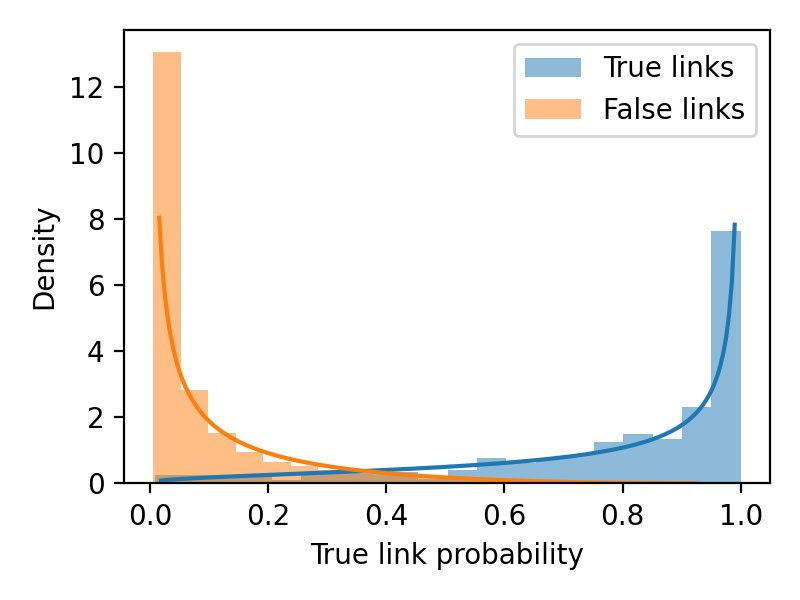
\includegraphics[width=\linewidth]{img/links_score_density_fusion_regression.png}

  \vspace{0.5cm}

  \subcaption{Z-Score fusion}
  \label{fig:links_score_density_fusion_z_score}
  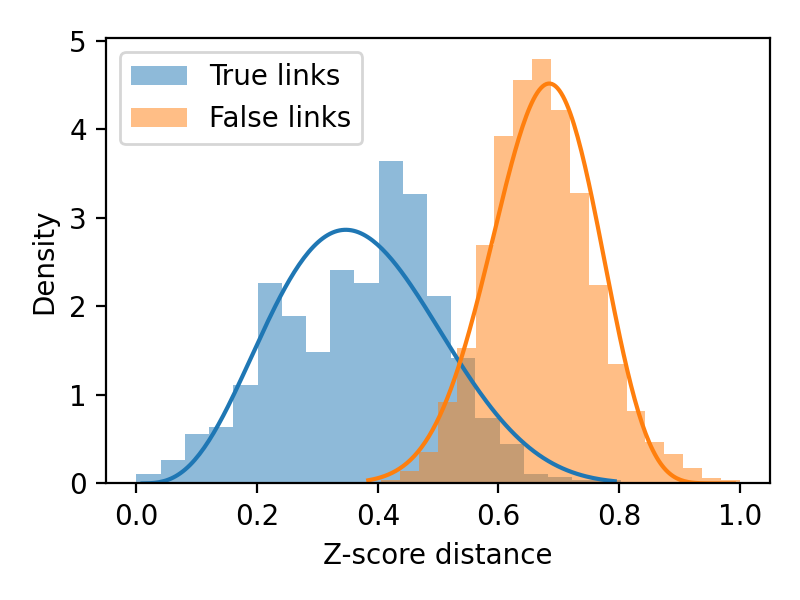
\includegraphics[width=\linewidth]{img/links_score_density_fusion_z_score.png}
\end{figure}

\subsubsection{Supervised distance threshold selection using Logistic Regression}

To learn at which position in the rank list the cut should be, this third idea is to fit a linear model on samples created from the rank list.
To train the model, a sample is created for each link in a rank list.
The links labels are either \textit{true} (1.0) when both document in the link are from the same author and \textit{false} (0.0) otherwise.
The features used are : the log of the relative rank ($log(\frac{rank}{|L|})$ and the score of the link.
Using these two features, the model can grasp the importance of the rank and the score of each link.
Since the training is only based on the relative rank and the score at each rank, the trained model is language independent and size independent.
But this model is metric dependent, since the score magnitude can variate depending on the distance function.

In this study, the model used is the logistic regression.
The advantage of using a regression model is that the output of the model will correspond to a probability of being a true link according to the model.
To find the cut on the test datasets, the fitted model predict the probability of being a true link on every link in the new rank list.
From these predictions a probability threshold must be chosen.
Having a probability threshold at $0.5$, minimize both false negatives and the false positives.
This can be adjusted, for example if false negatives are more important to minimize, a probability threshold at $0.6$ can be selected instead or $0.4$ if the false positive should be minimized.
For the sake of simplicity, the probability threshold chosen is $0.5$.

The distance threshold is chosen by linearly interpolating the probability threshold with its closest probability of the one above and the one below to their scores.
This ensures that the distance threshold chosen is even correct between ranks for any new corpus.
This is in particular useful when the training set is well separated (few links with probabilities around $0.5$) but the testing set is not.
Example~\ref{ex:linear_interpolation} show an example of linear interpolation computation using a probability threshold of $0.5$.
The logistic regression model can be re-used on any other rank lists produced with the same distance metrics.

\begin{example}
  \centering
  \caption{Linear interpolation for Supervised distance threshold selection}
  \label{ex:linear_interpolation}

  \begin{subexample}{\linewidth}
    \centering
    \subcaption{Rank list with link probability and score}
    \begin{tabular}{l r r}
      \toprule
      Rank & Probability & Score \\
      \midrule
      (...) & &\\
      45th & 0.54 & 15 \\
      46th & 0.52 & 13 \\
      47th & 0.49 & 12 \\
      48th & 0.48 & 10 \\
      (...) & & \\
      \bottomrule
    \end{tabular}
  \end{subexample}

  \vspace{0.5cm}

  \begin{subexample}{\linewidth}
    \centering
    \subcaption{Linear interpolation}
    \begin{align}
        \alpha &= \frac{0.5 - 0.49}{0.52 - 0.49} = \frac{1}{3} \\
        \textit{score}_{0.5} &= (13 - 12) \cdot \alpha + 12 = 12 + \frac{1}{3}
    \end{align}
  \end{subexample}

\end{example}
